\documentclass[a5paper]{article}
\usepackage[utf8]{inputenc}
\usepackage[T1]{fontenc}
\usepackage{txfonts}
\usepackage{bm}
\usepackage{geometry}
\usepackage{graphics}

\title{Statistics}
\author{Jon Hurst}

\begin{document}
\maketitle

\section{Measures of data}
\subsection{Mean and Variance}

If $f_i$ is the frequency that value $x_i$ occurs and $\overline{x}$ and
$\sigma^2$ are respectively the mean and variance for the frequency
distribution, then

\begin{equation}
  \overline{x} = \frac{\sum\limits_{all\ i} f_i x_i}{\sum\limits_{all\ i} f_i}
\end{equation}

\begin{equation} \label{eq:1}
  \sigma^2 = \frac{\sum\limits_{all\ i} f_i (x_i - \overline{x})^2}{\sum\limits_{all\ i} f_i}
\end{equation}

\noindent An alternative version of equation (\ref{eq:1}) can be derived by
multiplying out

\begin{equation}
  \frac{\sum\limits_{all\ i} f_i (x_i - \overline{x})^2}{\sum\limits_{all\ i} f_i} =
  \frac{\sum\limits_{all\ i} f_i x_i^2}{\sum\limits_{all\ i} f_i}
  -2\overline{x}\ \frac{\sum\limits_{all\ i} f_i x_i}{\sum\limits_{all\ i} f_i}
  + \overline{x}^2\ \frac{\sum\limits_{all\ i} f_i}{\sum\limits_{all\ i} f_i}
\end{equation}

\begin{equation} \label{eq:2}
  \Rightarrow\hspace{3em} \sigma^2 = \frac{\sum\limits_{all\ i} f_i x_i^2}{\sum\limits_{all\ i} f_i} -
  \overline{x}^2
\end{equation}

\noindent Equation (\ref{eq:2}) is sometimes verbalised as ``the mean of the squares
minus the square of the means''.

\subsection{Standard deviation}

Standard deviation, $\sigma$, is the square root of the variance. The advantage
of the standard deviation is that it has the same units as the mean.

\subsection{Weighted Mean}

The concept of a weighted mean is that some values are considered to be ``more
important'' to the mean than others. If we had, for example, a set of integer
values between 1 and 10 and we wanted 7 to be twice as important to the mean as
the other numbers, if each time 7 occurs we treat it as having occurred twice we
achieve the desired effect. In general, if we assign a weight, $w_i$, to each
possible value, then

\begin{equation}
  \overline{x} = \frac{\sum\limits_{all\ i} w_i f_i x_i}{\sum\limits_{all\ i}
    w_i f_i}
\end{equation}

Considering the above example, $w_i$ could be $1$ except for $w_7$ which would
be $2$. If $w_i$ were $\frac{1}{11}$ except for $w_7$ which would be
$\frac{2}{11}$, the result is the same because the $\frac{1}{11}$ factor can be
taken outside the summation signs for both numerator and denominator. The latter
scheme allows the total weight to add to 1, which is often how weights are
specified.

\section{Arrangements}

\subsection{Counting}

Consider all the ways that the numbers in the set \{1,2,3,4\} could be ordered.
One way to do this methodically would be with a tree diagram, as shown if Figure
\ref{fig:1}. The total number of possible arrangements is the number of entries
on the bottom line, and this can be seen to be $4\times 3\times 2\times 1 = 24$.
Essentially, there are 4 ways to fill the first number, then for each of those
4, 3 ways to fill the second number, then for each of those 3 only 2 ways to
fill the third number, with the last number being the only one remaining.

\begin{figure}[ht]

  \begin{center}
    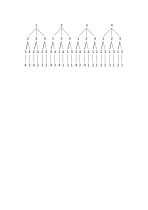
\includegraphics{arrangements}
  \end{center}
  \caption{Arrangements tree}
  \label{fig:1}
\end{figure}

This process can be generalised for $n$ numbers. The number of arrangements of
$n$ numbers will result from there being $n$ ways to fill the first number, then
for each of those $n$ ways, $(n-1)$ ways to fill the second number, continuing
until there is only one option for the final number. If $A_n$ is the number of
possible arrangements of $n$ numbers, therefore

\begin{equation} \label{eq:3}
  A_n = n!
\end{equation}

These numbers can, of course, represent any set of $n$ distinct objects -- if
they were physical objects you could always write the numbers on sticky labels
and attach them to the objects.

\subsection{Grouping}

Equation (\ref{eq:3}) gives the number of arrangements of distinct objects, but
what if some of the objects are indistinguishable from one another, e.g. you
wish to know how many arrangements can be made of 3 black balls and 2 white
balls, given that you can't tell the difference between balls of the same
colour?

The trick is to first label the objects, so that you \textit{can} tell the
difference, then group together the arrangements that \textit{would} be
indistinguishable without the labels. The answer is then the number of groups,
which can be calculated by dividing the total possible arrangements by the size
of a group.

In the example there are $5!$ ways of arranging the labelled balls, and each
grouping includes the $3!$ ways the black balls could be arranged and the $2!$
ways the white balls could be arranged that would result in indistinguishable
results (see Figure \ref{fig:2}).

\begin{figure}[ht]
  \begin{center}
    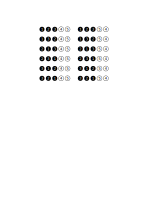
\includegraphics{arrangement-grouping}
  \end{center}

  \caption{Arrangement grouping}
  \label{fig:2}
\end{figure}

Thus the size of each group is $3!2!$, and the number of arrangements, given
that you can't tell the difference between balls of the same colour, is
$5!/(3!2!) = 10$.

\subsection{Rings}

If $n$ objects are arranged in a ring, and the orientation of the ring is
considered to be unimportant, then the size of the groupings of
indistinguishable arrangements is equal to the number of times the ring can be
rotated to give a new arrangement before it ends up back at the start. If there
are $n$ objects on the ring, therefore, the size of the groupings is $n$.
Hence, if $R_n$ is the number of distinguishable arrangements on a ring

\begin{equation}
  R_n = \frac{n!}{n} = (n-1)!
\end{equation}

If the ring may also be flipped, with all possible rotated arrangements in the
flipped state also to be considered indistinguishable, then the size of the
groupings is $2n$, and the number of distinguishable arrangements is $R_n / 2$.

\subsection{Permutations and Combinations}

The number of permutations, ${}^nP_r$, is the number of possible arrangements
resulting from selecting $r$ objects from a set of $n$ objects. The number of
ways of arranging the $n$ objects is $n!$, but only the first $r$ objects are
distinguishable. This means that the arrangements can be grouped by
considering all sub-arrangement of the remaining $(n-r)$ objects to be
indistinguishable, i.e. the group size is $(n-r)!$. Thus

\begin{equation}
  {}^nP_r = \frac{n!}{(n-r)!}
\end{equation}

The number of combinations, ${}^nC_r$, is the number of permutations but
considering order to be unimportant. This means the groupings of arrangements
include not only all possible sub-arrangements of the remaining $(n-r)$ objects,
but also all possible sub-arrangements of the $r$ selected objects. Thus the
group size is $r!(n-r)!$ and hence

\begin{equation}
  {}^nC_r = \frac{{}^nP_r}{r!} = \frac{n!}{(n-r)!r!}
\end{equation}

\section{Probability}
\subsection{Conditional probability}

$P(A\,|\,B)$ is the probability that an event A occurs given that an event B also
occurs. To calculate it, restrict the possibility space to only those outcomes
in which B occurs and consider how many times A also occurs.

\begin{equation} \label{eq:4}
  P(A\,|\,B) = \frac{P(A\cap B)}{P(B)}
\end{equation}

Since $P(A\cap B) = P(B\cap A)$ this also gives us

\begin{equation} \label{eq:5}
  P(A\,|\,B)P(B) = P(B\,|\,A)P(A)
\end{equation}
\subsection{Independent events}

Events A and B are independent if the occurrence of event B does not affect the
probability that A also occurs, i.e.

\begin{equation}
  P(A\,|\,B) = P(A)\hspace{3em} \mathrm{and}\hspace{3em} P(B\,|\,A) = P(B)
\end{equation}

Substituting equation (\ref{eq:4}) gives, \textit{for independent events only}

\begin{equation}
  P(A\cap B) = P(A)P(B)
\end{equation}

\subsection{Mutually exclusive events}

Events are mutually exclusive if

\begin{equation}
  P(A\cap B) = 0
\end{equation}

\subsection{Exhaustive events}

Events are exhaustive if

\begin{equation}
  P(A\cup B) = 1
\end{equation}

\subsection{Non-occurrence}

If $P(A)$ is the probability that event A occurs, $P(A^\prime)$ is the
probability that A \textit{does not} occur. The following identities are useful

\begin{eqnarray}
  P(A) = P(A\cap B) + P(A\cap B^\prime) \\
  P(B) = P(B\cap A) + P(B\cap A^\prime) \\
  P(A^\prime \cap B^\prime) = 1 - P(A \cup B)
\end{eqnarray}

\subsection{Bayes Theorem}

\begin{figure}[t]
  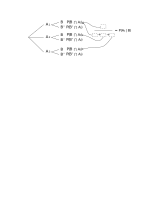
\includegraphics{bayes-theorem}

  \caption{Bayes Theorem}
  \label{fig:3}
\end{figure}


Rearranging equation (\ref{eq:5}) gives Bayes Theorem for two events

\begin{equation}
  P(A\,|\,B) = \frac{P(B\,|\,A)\ P(A)}{P(B)}
\end{equation}

\noindent If $A_i, i = 1, 2, 3, \ldots, n$ are $n$ exhaustive events then

\begin{equation}
  P(B) = \sum_{i=1}^{n} P(B\cap A_i)
\end{equation}

\begin{equation}
  \Rightarrow P(A_i\,|\,B) = \frac{P(B\,|\,A_i) P(A_i)}{\sum\limits_{j=1}^{n}P(B\,|\,A_j) P(A_j)}
\end{equation}

\noindent Figure \ref{fig:3} shows this relationship on a tree diagram.

\section{Discrete random variables}

\subsection{Definition}

A discrete random variable is a variable whose possible values are discrete
numerical outcomes of a random phenomenon. It embodies multiple possible values
simultaneously in the form of a probability mass function (PMF). You cannot
retrieve a value from a random variable, you can only retrieve the probability
that the outcome of the associated random phenomenon will either be a value or
be within a range of values.

\subsection{Operations}

Operations on a discrete random variable are transformations of the associated
probability mass function. For example if $X$ is a random selection of an
equally weighted integer in the range $[-2, 2]$ then its PMF is

\begin{equation}
  \begin{array}{c|ccccc}
    x & -2 & -1 & 0 & 1 & 2 \\[3pt]
    \hline \\[-8pt]
    P(X\!=\!x) & \frac{1}{5} & \frac{1}{5} & \frac{1}{5} & \frac{1}{5} & \frac{1}{5}
  \end{array}
\end{equation}

\noindent If $Y=X^2$ then $Y$ has PMF

\begin{equation}
  \begin{array}{c|ccc}
    x & 0 & 1 & 4 \\[3pt]
    \hline \\[-8pt]
    P(Y\!=\!x) & \frac{1}{5} & \frac{2}{5} & \frac{2}{5}
  \end{array}
\end{equation}

\noindent and if $Z = \frac{1}{2}(X - 1)$ its PMF is

\begin{equation}
  \begin{array}{c|ccccc}
    x & -\frac{3}{2} & -1 & -\frac{1}{2} & 0 & \frac{1}{2} \\[3pt]
    \hline \\[-8pt]
    P(Z\!=\!x) & \frac{1}{5} & \frac{1}{5} & \frac{1}{5} & \frac{1}{5} & \frac{1}{5}
  \end{array}
\end{equation}

\vbox{\noindent In general if $Y = g(X)$ then its PMF is

\begin{equation}
  \begin{array}{c|ccccc}
    x & g(-2) & g(-1) & g(0) & g(1) & g(2) \\[3pt]
    \hline \\[-8pt]
    P(Y\!=\!x) & \frac{1}{5} & \frac{1}{5} & \frac{1}{5} & \frac{1}{5} & \frac{1}{5}
  \end{array}
\end{equation}

with any duplicate values in the top line being combined.}

When dealing with functions of two random variables, you are dealing with a
three dimensional probability mass function. For example, if $X$ is defined as
above and $Y$ is a random integer in the range $[0,2]$ then if $Z = X + 2Y$, the
results table is

\begin{equation}
  \begin{array}{c|ccccc}
    y\backslash x & -2 & -1 & 0 & 1 & 2 \\[3pt]
    \hline \\[-8pt]
    0 & -2 & -1 & 0 & 1 & 2\\
    1 & 0 & 1 & 2 & 3 & 4\\
    2 & 2 & 3 & 4 & 5 & 6\\
  \end{array}
\end{equation}

Since both $X$ and $Y$ are random, i.e. the probability of any outcome is the
same, each outcome in the table has a probability of $\frac{1}{15}$. Combining
identical results we get

\begin{equation}
  \begin{array}{c|ccccccccc}
    x & -2 & -1 & 0 & 1 & 2 & 3 & 4 & 5 & 6\\[3pt]
    \hline \\[-8pt]
    P(Z\!=\!x) & \frac{1}{15} & \frac{1}{15} & \frac{2}{15} & \frac{2}{15} & \frac{3}{15}
    & \frac{2}{15} & \frac{2}{15} & \frac{1}{15} & \frac{1}{15}
  \end{array}
\end{equation}

\subsection{Expectation}

The expectation of a function $g$ of $X$ is defined as

\begin{equation} \label{eq:6}
  E(g(X)) = \sum_{all\ x} g(x)P(X\!=\!x)
\end{equation}
where $P(X\!=\!x)$ is the probability that the outcome of $X$ is $x$.

$E(X)$ is called the expected value of $X$. If $X_1, X_2, \ldots, X_n$ are $n$
independent random variables with PMF identical to $X$, then the mean of their
outcomes as $n\rightarrow\infty$ is equal to $E(X)$. E(X) is often written as
$\mu$.

$E((X-\mu)^2)$, often written as $Var(X)$, is called the variance of $X$. If
$X_1, X_2, \ldots, X_n$ are $n$ independent random variables with PMF identical
to $X$, then the variance of their outcomes as $n\rightarrow\infty$ is equal to
$Var(X)$.

An alternative form for variance is available by multiplying out $(X-\mu)^2$

\begin{eqnarray}
  E((X-\mu)^2) & = & \sum_{all\ x} (x-\mu)^2P(X\!=\!x) \nonumber\\
  & = &  \sum_{all\ x}x^2 P(X\!=\!x) - 2\mu\sum_{all\ x}x P(X\!=\!x) +
  \mu^2\sum_{all\ x}P(X\!=\!x) \nonumber\\
  & = & E(X^2) - E^2(X)
\end{eqnarray}

\subsection{Expectation arithmetic}

From equation (\ref{eq:6}), if $a$ and $b$ are constants then

\begin{equation}
  E(aX + b) = a\sum_{all\ x}xP(X\!=\!x)+ b\sum_{all\ x}P(X\!=\!x)  = aE(X) + b
\end{equation}

\begin{eqnarray}
  Var(aX + b) &=& E(a^2X^2 + 2abX + b^2) - (aE(X) + b)^2 \nonumber\\
  &=& a^2Var(X)
\end{eqnarray}
\noindent For discrete random variables $X$ and $Y$

\begin{eqnarray}
  E(aX + bY) & = & \sum_{all\,x}\sum_{all\,y}(ax + by)P(X\!=\!x,Y\!=\!y)\nonumber\\
  & = & a\sum_{all\,x}x\sum_{all\,y}P(X\!=\!x,Y\!=\!y)\nonumber\\
  & & \mbox{} + b\sum_{all\,y}y\sum_{all\,x} P(X\!=\!x,Y\!=\!y)\nonumber\\
  & = & a\sum_{all\,x}xP(X\!=\!x) + b\sum_{all\,y}yP(Y\!=\!y)\nonumber\\
  & = & aE(X) + bE(Y)
\end{eqnarray}

\begin{eqnarray} \label{eq:7}
  Var(aX + bY) & = & E(aX + bY)^2) - E^2(aX + bY) \nonumber\\
  &=& a^2(E(X^2) - E^2(X)) \nonumber\\
  & & \mbox{} + b^2(E(Y^2) - E^2(Y)) \nonumber\\
  & & \mbox{} + ab(E(XY) - E(X)E(Y))
\end{eqnarray}

\noindent The last term on the right of equation (\ref{eq:7}) is equal to zero
iff $X$ and $Y$ are \textit{independent}, in which case

\begin{equation}
  Var(aX + bY) = a^2Var(X) + b^2Var(Y)
\end{equation}

\section{Standard discrete distributions}

\subsection{Uniform distribution}

If a distribution is uniform, each result in the set $\{x_1, x_2, \ldots, x_n\}$ is
equally likely, i.e.

\begin{equation}
  P(X\!=\!x_i) = \frac{1}{n} \hspace{5em}\forall i \in 1, 2, \ldots, n
\end{equation}

\noindent Hence

\begin{equation}
  E(X) = \frac{1}{n}\sum_{all\,i}x_i
\end{equation}

\begin{equation}
  Var(X) = \frac{1}{n}\sum_{all\,i}x_i^2 - E^2(X)
\end{equation}

\subsection{Geometric distribution}

If $X$ is the number of independent trials to obtain the first successful
outcome, where the probability of a successful outcome is $p$, then $X$ is
distributed geometrically with parameter $p$ (written as $X\sim Geo(p)$) and

\begin{eqnarray}
  P(X\!=\!x) &=& (1-p)^{x-1}p \\
  P(X\!>\!x) &=& (1-p)^x \\
  P(X\!\leq\!x) &=& 1 - (1-p)^x
\end{eqnarray}

\begin{eqnarray}
  E(X) &=& \sum_{i=1}^\infty ip(1-p)^{i-1} \nonumber\\
  &=& p + \sum_{i=2}^\infty ip(1-p)^{i-1} \nonumber\\
  &=& p + (1-p)\sum_{i=2}^\infty [(i-1) + 1]p(1-p)^{i-2}]\nonumber\\
  &=& p + (1-p)\left[E(X) + 1\right]\nonumber
\end{eqnarray}

\begin{equation}
  \Rightarrow E(X) = \frac{1}{p}
\end{equation}

\begin{eqnarray}
  E(X^2) &=& \sum_{i=1}^\infty i^2p(1-p)^{i-1} \nonumber\\
  &=& p + (1-p)\sum_{i=2}^\infty [(i-1)^2 +2(i-1) +1]p(p-1)^{i-2} \nonumber\\
  &=& p + (1-p)[E(X^2) + 2E(X) + 1]\nonumber
\end{eqnarray}

\begin{equation}
  \Rightarrow E(X^2) = \frac{2 - p}{p^2}
\end{equation}

\begin{equation}
  \Rightarrow Var(X) = \frac{1 - p}{p^2}
\end{equation}

\subsection{Binomial distribution}

Let $X$ be the number of ``successful'' outcomes from a series of $n$
independent trials, where $p$ is the probability of a successful trial. Then $X$
has a binomial distribution, written $X \sim B(n,p)$ and

\begin{equation}
  P(X\!=\!r) = {}^nC_rp^r(1-p)^{n-r}
\end{equation}

A good way to think about this is to consider the series of trials as a
probability tree. Any path through the tree that results in $r$ successes has a
probability of $p^r(1-p)^{n-r}$. We then need to work out how many paths there
are through the tree that contain $r$ successes. To do this, we need to see how
many ways there are to choose $r$ of the $n$ trials to be successes, which is
${}^nC_r$.

To find the expected value and variance, we first need to consider variables
with the Bernoulli distribution. A Bernoulli variable has value $1$ with a
probability of $p$ and a value $0$ with a probability of $(1-p)$. If $A$ is a
Bernoulli variable


\begin{equation}
  E(A) = 0(1-p) + 1(p) = p \\
\end{equation}
\begin{equation}
  E(A^2) = 0^2(1-p) + 1^2(p) = p \\
\end{equation}
\begin{equation}
  Var(A) = p(1-p)
\end{equation}

If $X\sim B(n,p)$ and $A_1, A_2, \ldots, A_n$ are $n$ independent identically
distributed Bernoulli trials with probability of success $p$ then

\begin{equation}
  X = \sum_{i=1}^n A_i
\end{equation}

Hence

\begin{equation}
  E(X) = nE(A_1) = np
\end{equation}
\begin{equation}
  Var(X) = nVar(A_1) = np(1-p)
\end{equation}

\subsection{Poisson distribution}

The Poisson distribution is the limiting case of the Binomial distribution when
$n\rightarrow\infty$ and $np = \lambda$ where $\lambda$ is a constant used as
the distribution parameter. If $X\sim Po(\lambda)$

\begin{equation}\label{eq:8}
  P(X\!=\!k) = \lim_{n
    \rightarrow\infty}{}^nC_r\left(\frac{\lambda}{n}\right)^k
  \left(\left(1 + \frac{-\lambda}{n}\right)^{\frac{n-k}{-\lambda}}\right)^{-\lambda}
\end{equation}

\begin{equation}\label{eq:9}
  \lim_{n\rightarrow\infty}\frac{{}^nC_r}{n^k} =
  \lim_{n\rightarrow\infty}\frac{(n)(n-1)(n-2)\ldots(n-k+1)}{n^k} = 1
\end{equation}

Substituting equation (\ref{eq:9}) into equation (\ref{eq:8}) and recognising
that the limit of the rightmost term of equation (\ref{eq:9}) is $e^{-\lambda}$

\begin{equation}
  P(X\!=\!k) = \frac{\lambda^k}{n!}e^{-\lambda}
\end{equation}

Since the Poisson distribution is the limiting case of the Binomial
distribution, the expected value and variance are found by substituting $np =
\lambda$ and $(1-p) = 1$ into the equations of the Binomial

\begin{equation}
  E(X) = \lambda
\end{equation}
\begin{equation}
  Var(X) = \lambda
\end{equation}

The Poisson distribution can be used as a good approximation for the Binomial
distribution if $n$ is large and $p$ is small. The textbook gives \mbox{$n\ge 50$} and
$p\le 0.1$ as suitable cutoffs.
\end{document}
